\chapter{Results And Discusions}
This chapter presents the results obtained from the series of algorithms implemented in python and detailed discussions of the results are also presented. 
\section{Words occurrence in the Documents}
Prior to plotting figure \eqref{Fig. 4.1} the top ten occurring words in the dictionary of the 1259 text documents are "red", "cross",  "support", "ifrc", "national", "activities","operation", "volunteers", "people" and "emergency". These words were removed because they are perceived  to be often used in almost all the text documents, considering the nature of the reports and the source. In other words they are key words that are always used in reporting events concerning disaster and  related issue. Even though there is no clear motive for removing these words, one reason thought to be convincing is that these words repeats more frequently in almost all the topics when trained on  the LDA model, however these repetitions may be viewed to make sense because the reports talks about similar issues. These repetition effect continued even after the initial top words in the documents were removed, but  the repetitions decreased with the next set of frequently occurring words.
\begin{figure}[hbtp]
\centering
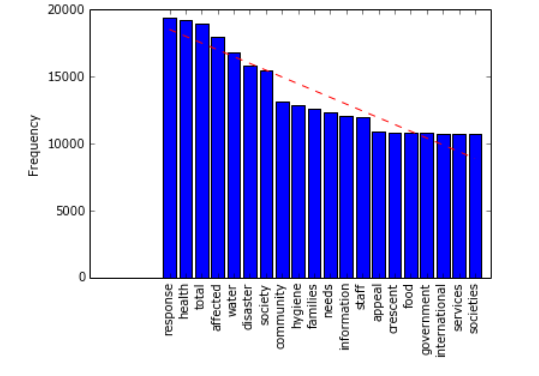
\includegraphics[scale=0.80]{c4_1.png}
\caption{Top 10 words  in the text collections}\label{Fig. 4.1}
\end{figure}
 
\section{Topics Distribution over words}
Table \eqref{Table 4.1} shows 11 topics selected out of the 30 topics the LDA model produced when trained on the data. 
Topic number 7, 10, 13, 14, and 18 can be considered to describe cash transfer programs (CTP). Food, cash and shelter are some forms of CTP's given to victims who have suffered  a disaster event. Some  reports out of the 1259 text files are CTP reports. It is very likely that these topics are associated with these particular set of reports. Topic 18 particularly relates to documents describing the source of the CTP's. The "sarc" word in this topic is an abbreviation that stands for Syrian Arab Red Crescent, a humanitarian NGO (private) that provides some form of  CTP to victims.

Topic 19 is distributed over words such as "krcs", "kenya", "nairobi", "garrisa. krcs means Kenya red cross crescent society, nairobi is Kenya's capital city. It can be inferred that there exist a document or some number of documents contained in the reports that talks about kenya, probably about disease related disaster outbreaks. 

The term "mena" in topic 27 is an acronym for countries in Middle East and Northern Africa. The other words occurring together with "mena" in this topic such as "syrian", "lebanon",and "iraq" are terms related to countries that falls in the domain of MENA. For easy query of documents or reports in relation to countries of MENA, topic 27 can be used to trace and easily find such documents.

Topic 28 has 3 very common disease outbreaks that affected some countries across the globe. The "zika", "cholera", and "chikungunya". The chikungunya and zika diseases spread are associated with mosquitoes, and the Dominican republic has been hit with the zika and chikungunya diseases. 
\begin{figure}[hb]
\centering
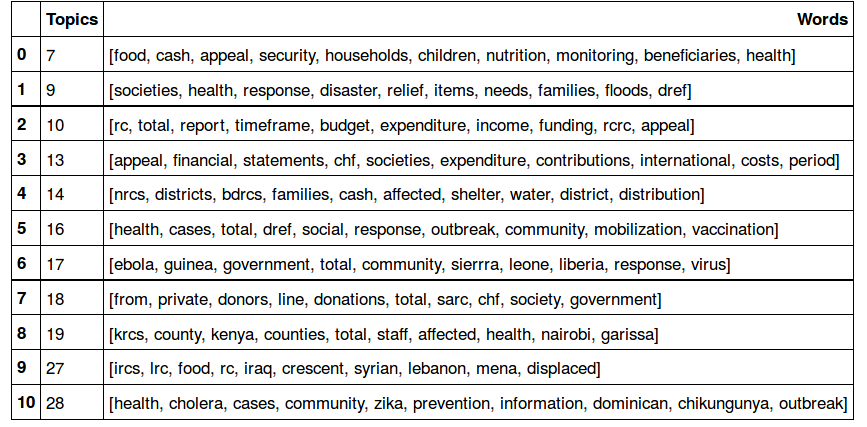
\includegraphics[scale=0.6]{c4_2.png}
\caption{Top 11 topics from the trained LDA model.}
\end{figure}\label{Table 4.1}
\section{Documents distribution over topics}
The trained LDA model revealed that several topics in related to the various documents used to train the model. Figure \eqref{Figure 4.2} shows the extent to which a document can exhibits multiple topics. Each of the vertically rectangular bar corresponding to a document is consist of rectangles in it, of which each is a topic. That is each bar consist of rectangles. All the ten documents in \eqref{Figure 4.2} exhibits more than one topic. Document 7 is distributed over 10 topics with documents 2 and 5 having the least number of topics distribution,  they have two topics each. The sum of the probabilities for each bar of its constituent rectangle values adds up to 1.
\begin{figure}[h]
\centering
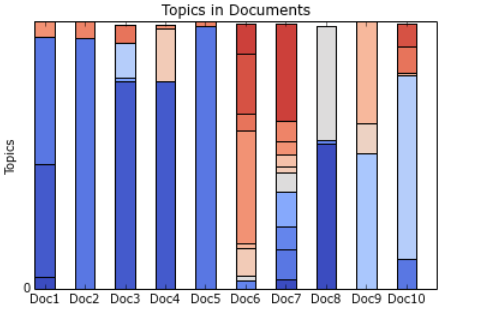
\includegraphics[scale=0.85]{c4_3.png}
\caption{Stacked graph of topics composition in documents}\label{Figure 4.2}
\end{figure}
\section{Topics Concentration in Documents}
The LDA topic model does not just inform us about the fact documents constitutes multiple topics, but also tells us the proportion and how concentrated the topics are in each of the documents. From \eqref{Figure 4.3} the blue coloured rectangles varies with intensity. As shown in the the probability scale on the right of \eqref{Figure 4.3}, deeply coloured means high probability $(0.9-1)$, in that order. It is observed that topic 3 are highly in documents 2 and 5. The proportion of topics 3,4,7,15,18, 19, 23 and 24 occur in small proportions in document 7.
\begin{figure}[hbtp]
\centering
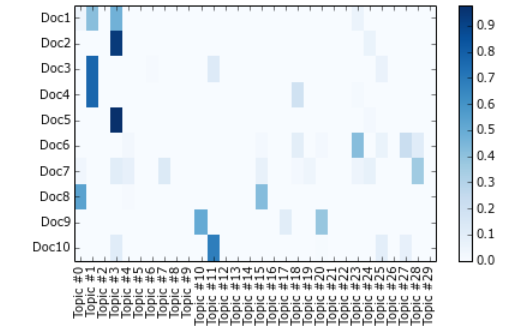
\includegraphics[scale=0.85]{c4_4.png}
\caption{Heat graph showing topics concentration in documents.}\label{Figure 4.3}
\end{figure}
\newpage
\section{Topics and Documents relationship}
\begin{flushleft}
In topic modelling the documents constituting the corpus may arise from one subject area or may not. The nature of the distribution of the terms in each of the topics can predict how the documents collection are related. That is to say if some of the terms are are found in many topics, then the topics can be said to be  related and hence the documents. 
\end{flushleft}
\begin{flushleft}
Considering figure \eqref{figure 4.5} the circles (0-29) are the topics and on the right are the terms constituents of each topic. This implies that red circle (topic 26) is composed of the words "appeal" down to "allocations", these words are the top most 30 terms connected to topic 26.
\end{flushleft}
\begin{flushleft}
The size of the circle also tells how prevalent it is in the corpus. That is, the bigger the circle the more prevalent that topic is in the documents. Figure \eqref{Table 4.5} shows how frequent topic 1 occurs in the documents more than the other 29 topics.
\end{flushleft}
\begin{flushleft}
The map  also also reveals the semantic distances between the topics. From \eqref{figure 4.5} it shows that nineteen of the topics are crowded in one region, the extreme  right end of the horizontal axes. This means that more than $50\%$ of the topics are similar and hence gives an indication that, most of documents in the corpus share similar topics.
\end{flushleft}
\begin{figure}[h!]
    \centering
    \begin{subfigure}[h]{0.60\textwidth}
        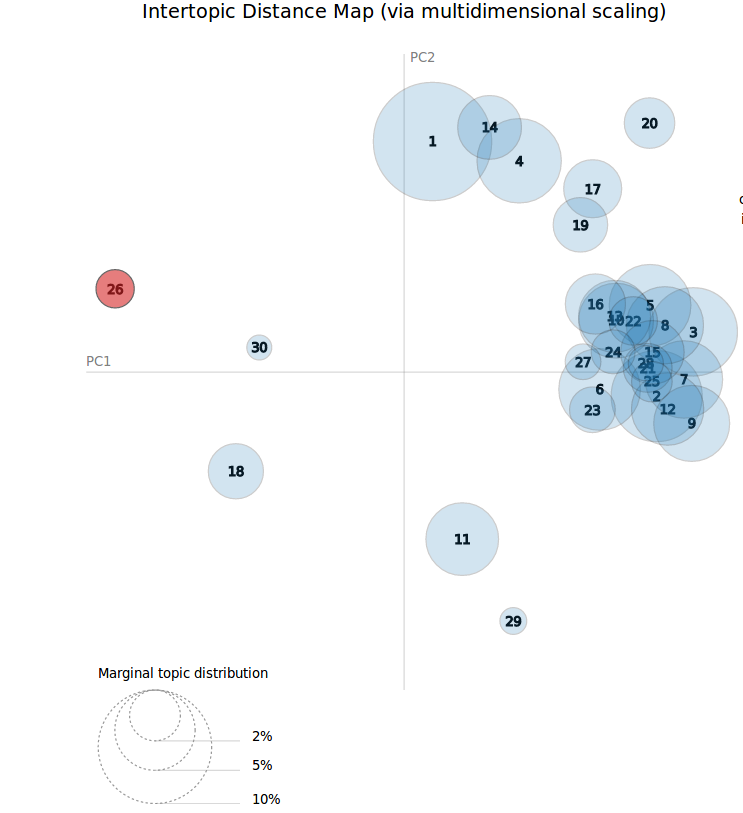
\includegraphics[width=\textwidth]{c4_5.png}
        \caption{Map of the 30 topics from LDA model.}
        \label{fig:trapez1}
    \end{subfigure}
    ~ %add desired spacing between images, e. g. ~, \quad, \qquad, \hfill etc. 
      %(or a blank line to force the subfigure onto a new line)
    \begin{subfigure}[h]{0.60\textwidth}
        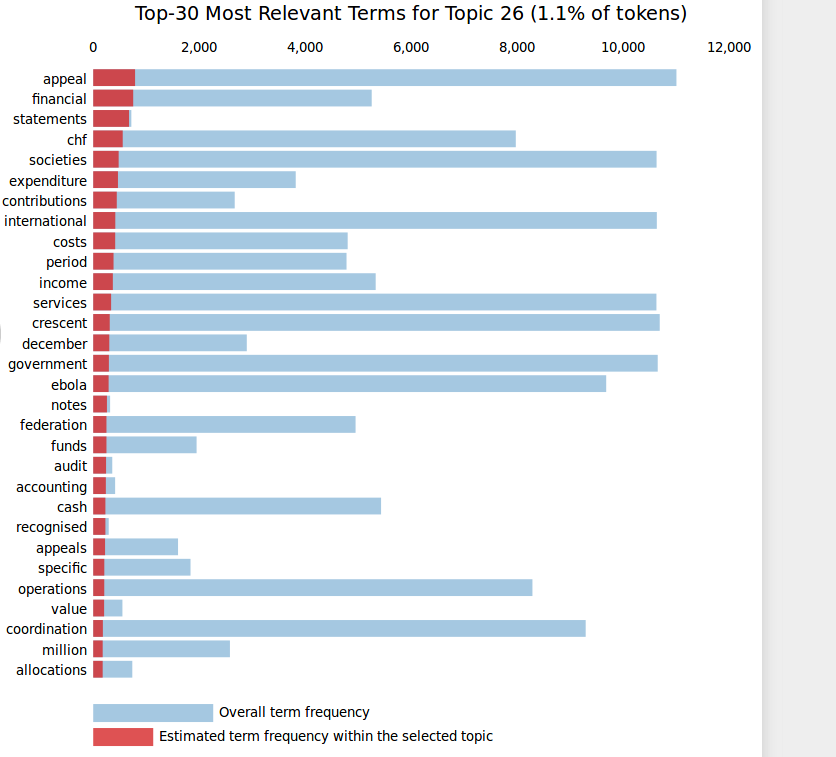
\includegraphics[width=\textwidth]{c4_6.png}
        \caption{Prevalence of words in topics and in the corpus.}
        \label{fig:trapez2}
    \end{subfigure}
    \caption{LDAvis for topics and words distribution}\label{figure 4.5}
\end{figure}
\newpage
\begin{figure}[h!]
    \centering
    \begin{subfigure}[h]{0.60\textwidth}
        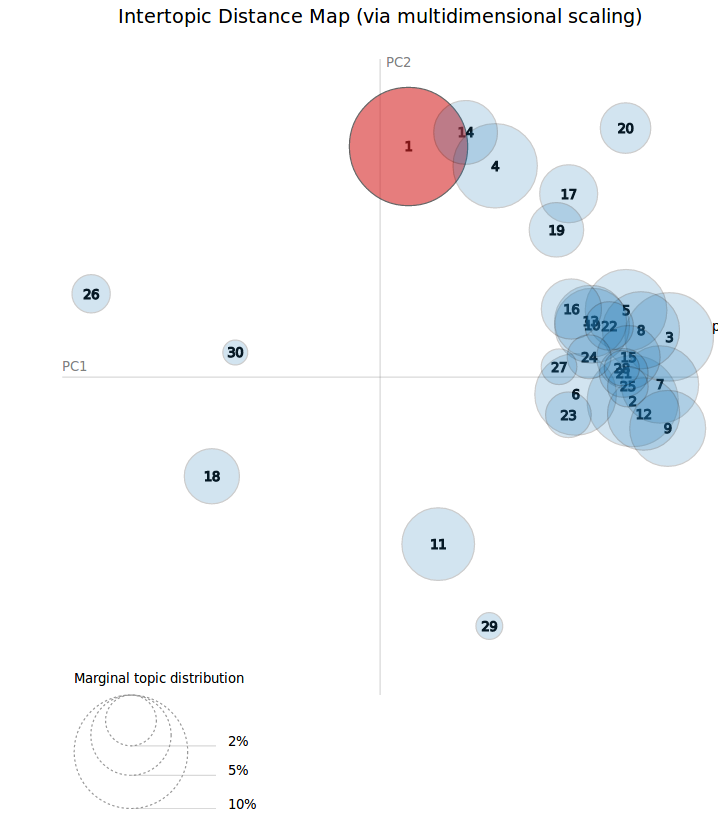
\includegraphics[width=\textwidth]{c4_7.png}
        \caption{Map of the 30 topics from LDA model.}
        \label{fig:trapez1}
    \end{subfigure}
    ~ %add desired spacing between images, e. g. ~, \quad, \qquad, \hfill etc. 
      %(or a blank line to force the subfigure onto a new line)
    \begin{subfigure}[h]{0.60\textwidth}
        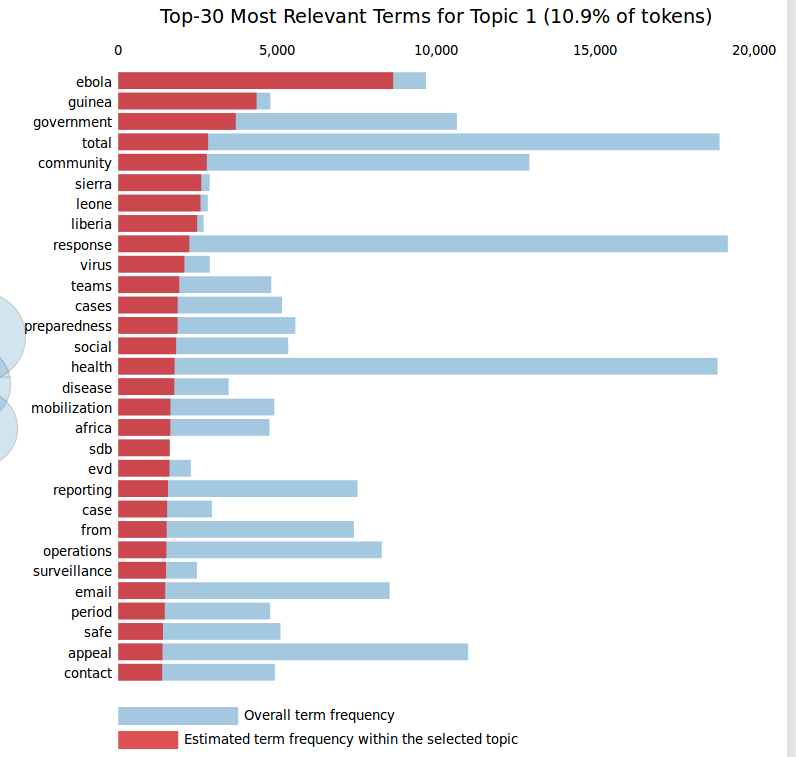
\includegraphics[width=\textwidth]{c4_8.png}
        \caption{Prevalence of words in topics and in the corpus.}
        \label{fig:trapez2}
    \end{subfigure}
    \caption{LDAvis for topics and words distribution}\label{figure 4.6}
\end{figure}
%An average essay may contain five chapters, but I didn't plan my work properly
%and then ran out of time. I spent too much time positioning my figures and worrying
%about my preferred typographic style, rather than just using what was provided.
%I wasted days bolding section headings and using double slash line endings, and 
%had to remove them all again. I spent sleepless nights configuring manually numbered lists
%to use the \LaTeX\ environments because I didn't use them from the start or understand
%how to search and replace easily with texmaker.
%
%Everyone has to take some shortcuts
%at some point to meet deadlines. Time did not allow to test model 
%B as well. So I'll skip right ahead and put that under my Future Work section.


%\section{This is a section} 
%Text text text text text text text text text text text text text text
%text text text text text text text text text text text text text text
%text text text text text text text text text text text text text text
%text text text text text text text text text text text text text text
%text text text text text. 
%
%Some essays may have 3, 5 or 6 chapters. This is just an example. 
%More importantly, do you have at most 35 pages?  
%Luck has nothing to do with it. Use the techniques suggested for
%writing your essay.
%
%Now you're demonstrating pure talent and newly acquired skills. 
%Perhaps some persistence. Definitely some inspiration. What was that about perspiration? 
%Some team work helps, so every now and then why not browse your friends' essays and provide
%some constructive feedback?
